% !TeX program = xelatex
% !TeX encoding = UTF-8
\documentclass[aspectratio=169,11pt]{beamer}

\usepackage{fontspec}
\usepackage{polyglossia}
\setdefaultlanguage{vietnamese}
\IfFontExistsTF{Arial}{\setsansfont{Arial}}{\setsansfont{Liberation Sans}}
\IfFontExistsTF{Times New Roman}{\setmainfont{Times New Roman}}{\setmainfont{Liberation Serif}}
\usefonttheme{professionalfonts}

\usepackage{amsmath,amssymb}
\usepackage{booktabs}
\usepackage{graphicx}
\usepackage{array}
\usepackage{xcolor}
\usepackage{hyperref}

\usetheme{Madrid}
\setbeamertemplate{navigation symbols}{}
\setbeamertemplate{footline}[frame number]

\newcommand{\figmaybe}[2]{%
  \IfFileExists{#1}{\includegraphics[width=#2]{#1}}{\fbox{\parbox[c][0.42\textheight][c]{#2}{\centering Chạy code để sinh hình\\\texttt{\detokenize{#1}}}}}
}

\title{Dự đoán nguy cơ đột quỵ bằng XGBoost, PCA và XAI}
\subtitle{Tái hiện nghiên cứu Mochurad et al. (2025)}
\author[Nhóm thực hiện]{
	\small
	\textbf{Học phần:} HỌC MÁY VÀ KHAI PHÁ DỮ LIỆU \\[0.2cm]
	\textbf{Giảng viên hướng dẫn:} TRẦN TRỌNG HIẾU \\[0.8cm]
	\textbf{Học viên thực hiện:} \\[0.2cm]
	1. TỐNG VIỆT TÚ - Mã học viên: 25007845 \\[0.15cm]
	2. NGUYỄN THỊ NHẬT LINH - Mã học viên: 25007871
}

\date{\today}

\begin{document}

\begin{frame}
  \titlepage
\end{frame}

\begin{frame}{1. Bài toán và động cơ}
\begin{itemize}
  \item Mục tiêu: dự đoán sớm nguy cơ đột quỵ từ đặc trưng bệnh nhân.
  \item Khó khăn: \textbf{mất cân bằng lớp} (chỉ 4.3--4.9\% ca dương tính), missing/outlier, quan hệ phi tuyến, yêu cầu giải thích.
  \item Hướng của bài báo: \textbf{XGBoost + PCA + SHAP}; PCA được tối ưu bằng OpenMP.
\end{itemize}
\begin{block}{Ba tiêu chí chính}
Độ chính xác \quad + \quad tốc độ xử lý \quad + \quad khả năng giải thích.
\end{block}
\end{frame}

\begin{frame}{2. Hai bộ dữ liệu}
\small
\begin{tabular}{p{0.24\linewidth}p{0.22\linewidth}p{0.46\linewidth}}
\toprule
\textbf{Bộ dữ liệu} & \textbf{Quy mô} & \textbf{Đặc trưng chính}\\\midrule
Dataset 1 & 5,110 bản ghi; 249 stroke (4.87\%) & age, hypertension, heart disease, glucose, BMI, smoking, work type, gender, residence\\
Dataset 2 & 5,542,261 bản ghi; 235,961 stroke (4.26\%) & Cấu trúc tương tự, dữ liệu tổng hợp quy mô lớn\\
\bottomrule
\end{tabular}
\vspace{0.5em}
\begin{itemize}
  \item Chia 80/20 (stratified) cho cả hai tập; sau tiền xử lý (one-hot) đều có \textbf{21 đặc trưng đầu vào}.
  \item Dataset 1: cân bằng bằng \textbf{SMOTE}.
  \item Dataset 2: cân bằng bằng \textbf{random undersampling}.
\end{itemize}
\end{frame}

\begin{frame}{3. Pipeline của nghiên cứu}
\centering
\begin{minipage}{0.84\linewidth}
\begin{enumerate}
  \item Làm sạch, missing, outlier, one-hot encoding.
  \item Chuẩn hóa dữ liệu.
  \item Cân bằng lớp trên tập train (trong pipeline, tránh rò rỉ dữ liệu).
  \item PCA giữ $\ge 95\%$ phương sai (Jacobi + OpenMP).
  \item XGBoost + tuning hyperparameter (Grid Search, Stratified K-Fold).
  \item Đánh giá: Accuracy, Precision, Recall, F1, ROC-AUC, MCC, Cohen's Kappa.
  \item XAI bằng SHAP (Waterfall, Bar, Beeswarm).
\end{enumerate}
\end{minipage}
\end{frame}

\begin{frame}{4. PCA: giảm chiều}
\[
X_c=X-\bar{x},\qquad
S=\frac{1}{N-1}X_c^TX_c,
\]
\[
Sv_j=\lambda_jv_j,\qquad X_{\text{reduced}}=X_cV_k.
\]
\begin{itemize}
  \item Chọn $k$ sao cho cumulative explained variance đạt $\ge$95\%.
  \item Theo bài báo: từ \textbf{21} đặc trưng sau tiền xử lý xuống còn \textbf{11} thành phần chính (cả hai tập dữ liệu).
  \item Phương sai giải thích đạt \textbf{96.90\%} (Dataset 1) và \textbf{96.96\%} (Dataset 2).
  \item Jacobi rotation được song song hóa bằng OpenMP.
\end{itemize}
\end{frame}

\begin{frame}{5. XGBoost và hàm mục tiêu}
\[
L(\theta)=\sum_{i=1}^{N}\ell(y_i,\hat y_i(\theta))+\Omega(\theta)
\]
\[
\ell(y_i,\hat y_i)=-\big[y_i\log\hat y_i+(1-y_i)\log(1-\hat y_i)\big].
\]
\begin{itemize}
  \item Tuning: depth, learning rate, số cây, gamma, min child weight, subsample, colsample.
  \item Regularization giúp kiểm soát overfitting.
  \item ROC-AUC là tiêu chí quan trọng khi lựa chọn mô hình (Grid Search + Stratified K-Fold).
\end{itemize}
\end{frame}

\begin{frame}{6.1. Kết quả PCA (Dataset 1)}
	\begin{columns}[T]
		% Cột bên trái
		\begin{column}{0.48\textwidth}
			\centering
			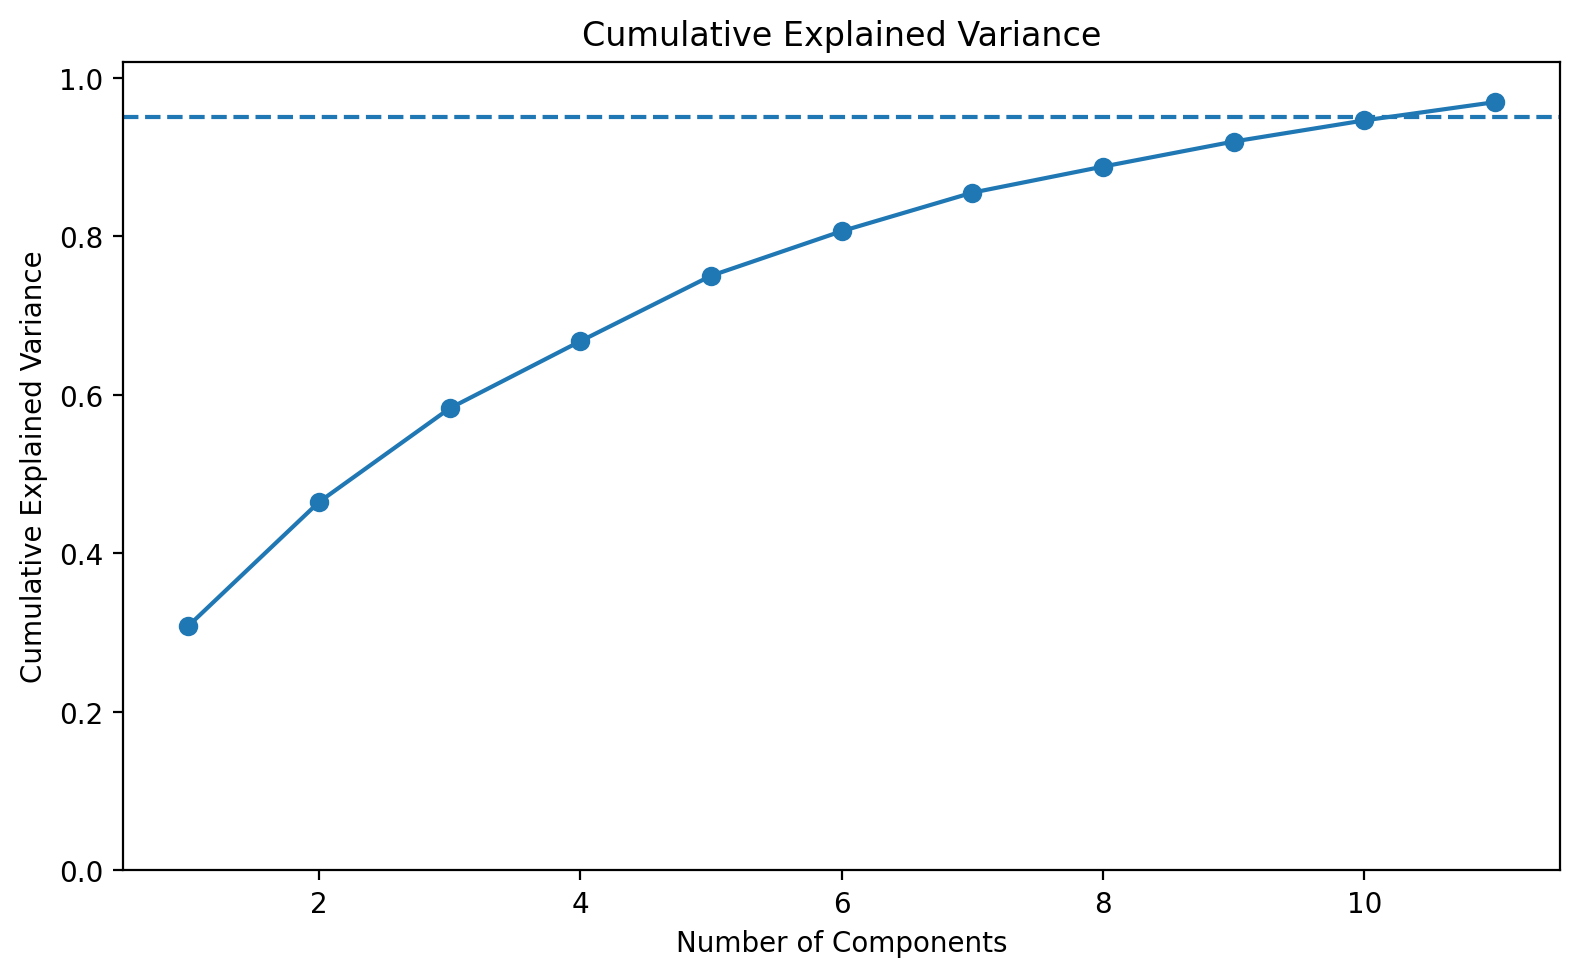
\includegraphics[width=0.95\linewidth]{figures_original/ds1-cumulative_variance.png}
			\par\vspace{0.2cm} % Tạo khoảng trống nhỏ giữa hình và chữ
			{\small Phương sai tích lũy theo thành phần\par}
		\end{column}
		
		% Cột bên phải
		\begin{column}{0.48\textwidth}
			\centering
			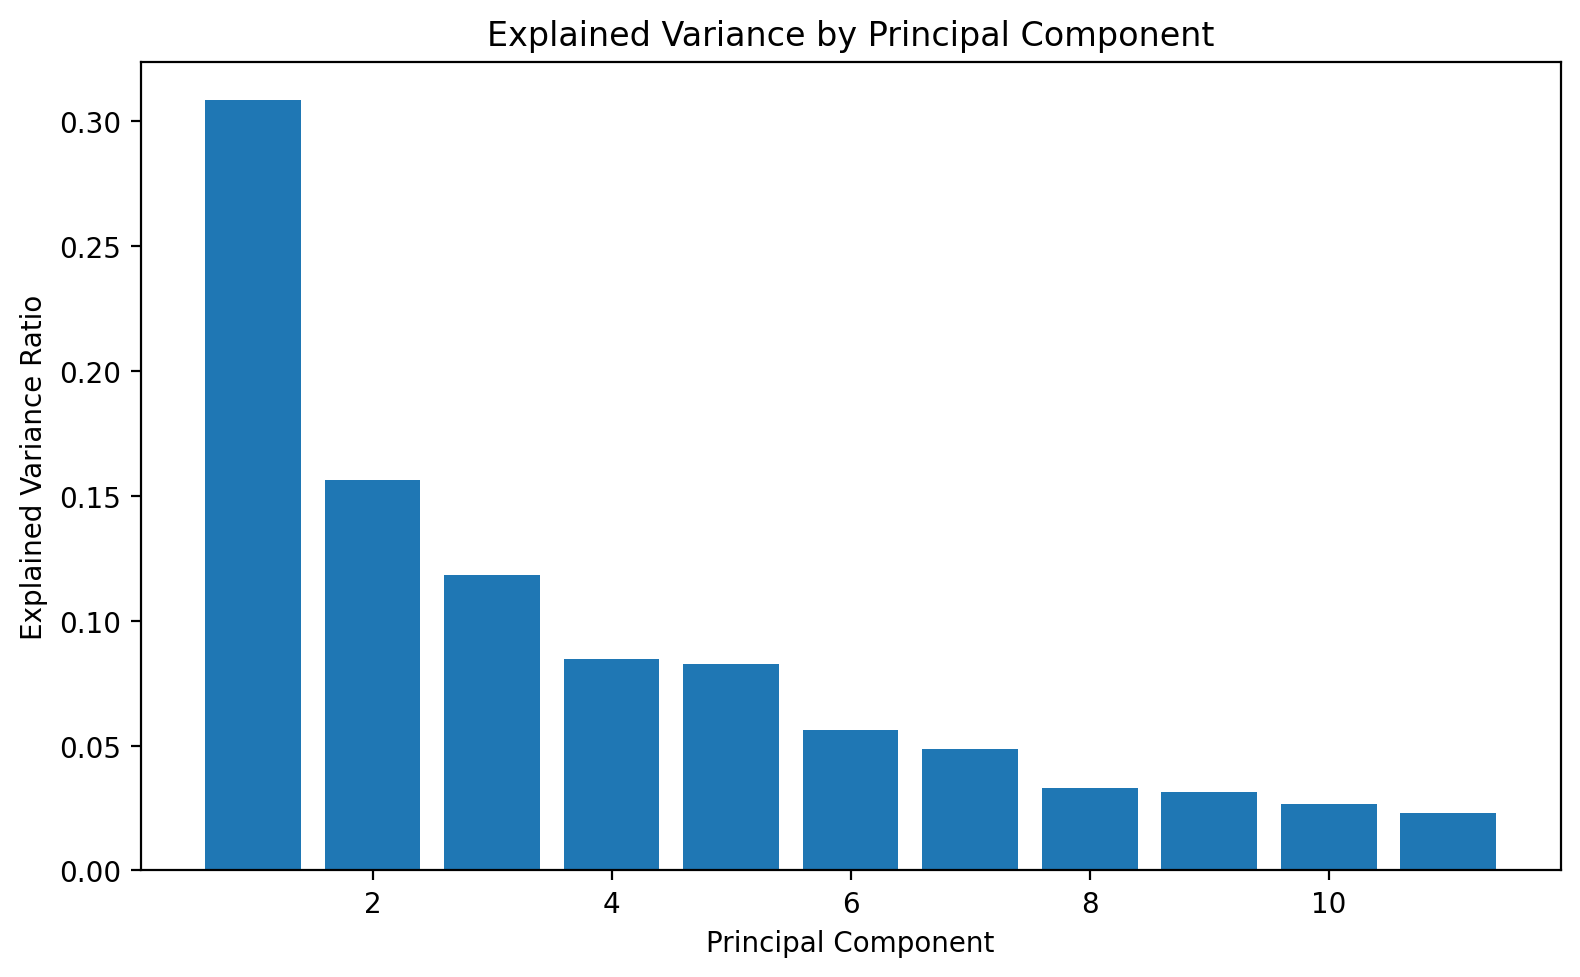
\includegraphics[width=0.95\linewidth]{figures_original/ds1-explained_variance.png}
			\par\vspace{0.2cm}
			{\small Tỷ lệ phương sai từng thành phần\par}
		\end{column}
	\end{columns}
\end{frame}

\begin{frame}{6.2. Kết quả PCA (Dataset 2)}
	\begin{columns}[T]
		% Cột bên trái
		\begin{column}{0.48\textwidth}
			\centering
			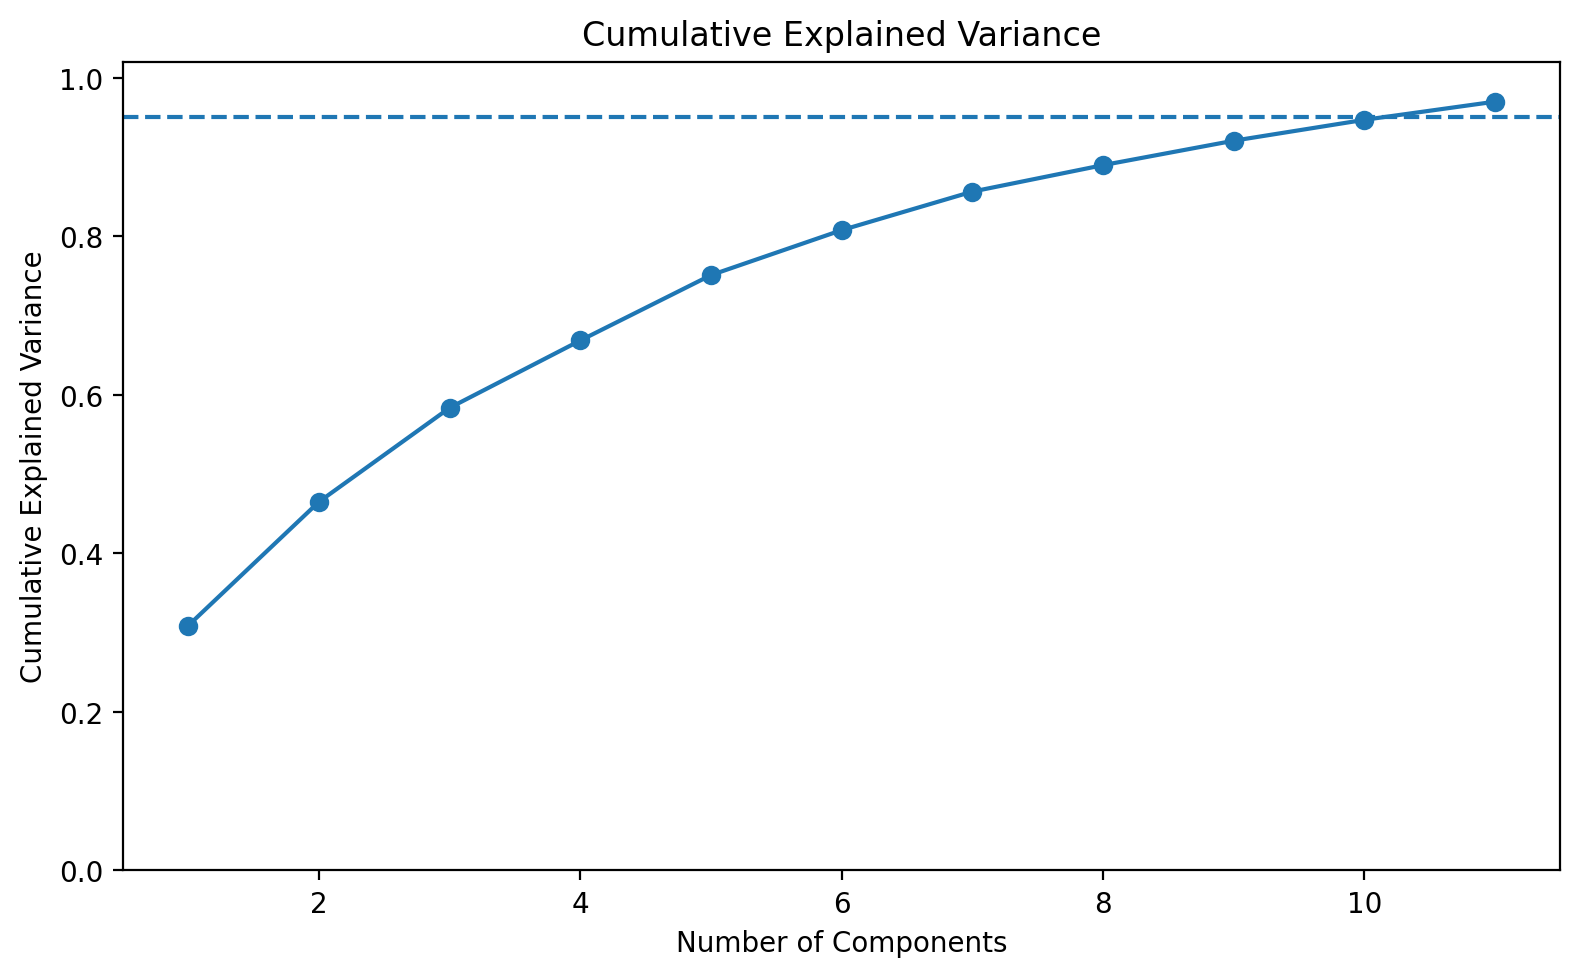
\includegraphics[width=0.95\linewidth]{figures_original/ds2-cumulative_variance.png}
			\par\vspace{0.2cm} % Tạo khoảng trống nhỏ giữa hình và chữ
			{\small Phương sai tích lũy theo thành phần\par}
		\end{column}
		
		% Cột bên phải
		\begin{column}{0.48\textwidth}
			\centering
			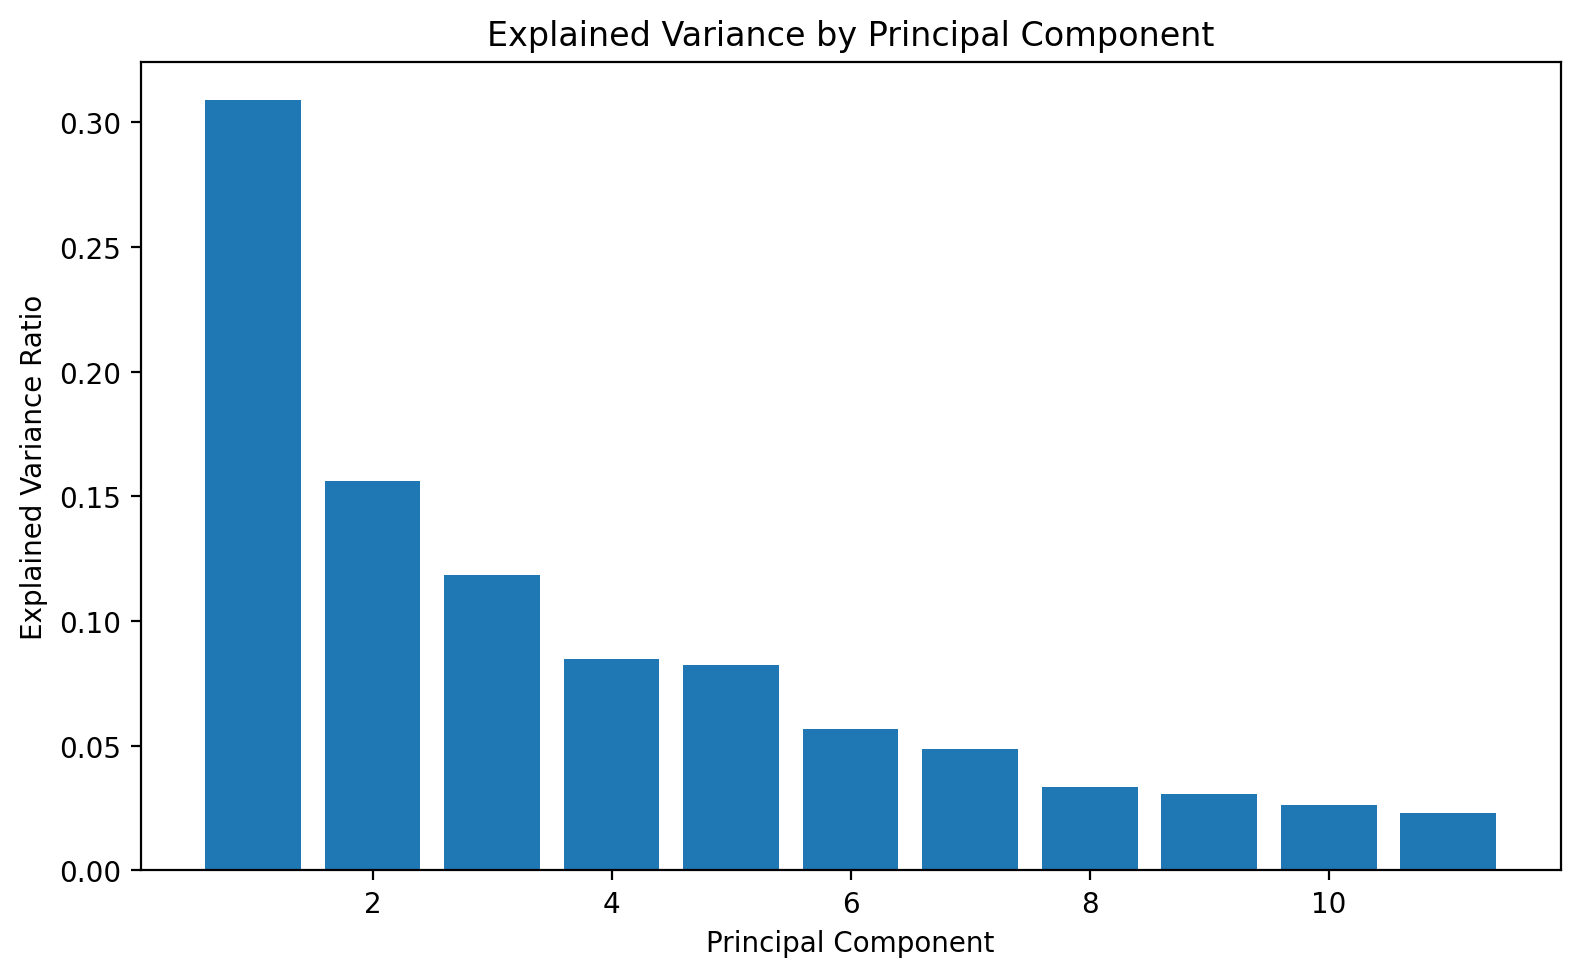
\includegraphics[width=0.95\linewidth]{figures_original/ds2-explained_variance.png}
			\par\vspace{0.2cm}
			{\small Tỷ lệ phương sai từng thành phần\par}
		\end{column}
	\end{columns}
\end{frame}

\begin{frame}{7. Hiệu năng mô hình baseline trên tập kiểm tra}
	
	\begin{columns}[T]
		
		% ==================== BÊN TRÁI ====================
		\column{0.40\textwidth}
		
		\begin{itemize}
			\item Mô hình đạt \textbf{Accuracy cao} trên cả 4 tập dữ liệu
			(0.9491--0.9638).
			\item Tuy nhiên, \textbf{Recall lớp 1 thấp}, chỉ từ
			0.0400 đến 0.1538.			
			\item Nguyên nhân: do tỷ lệ lớp dương thấp (4.3-4.9%).
			\item \textbf{Nhận xét:} Để tăng khả năng dự báo,
			\begin{itemize}
				\item Ngoài Accuracy, cần bổ sung Precision, Recall, F1-score  hay AUC-ROC
				\item Nên áp dụng các kỹ thuật cân bằng dữ liệu + tinh chỉnh siêu tham số.
			\end{itemize}
		\end{itemize}
		
		
		% ==================== BÊN PHẢI ====================
		\column{0.60\textwidth}
		
		\centering
		
		\scriptsize
		
		\renewcommand{\arraystretch}{1.35}
		
		\begin{tabular}{lcccc}
			\hline
			\textbf{Chỉ tiêu}
			& \textbf{D1--} 
			& \textbf{D1--}
			& \textbf{D2--}
			& \textbf{D2--} \\
			& \textbf{không PCA}
			& \textbf{có PCA}
			& \textbf{không PCA}
			& \textbf{có PCA} \\
			\hline
			
			Accuracy
			& 0.9501
			& 0.9491
			& 0.9612
			& \textbf{0.9638} \\
			
			Precision (lớp 1)
			& 0.4286
			& 0.3333
			& 0.9152
			& \textbf{0.9723} \\
			
			Recall (lớp 1)
			& 0.0600
			& 0.0400
			& 0.0986
			& \textbf{0.1538} \\
			
			F1 (lớp 1)
			& 0.1053
			& 0.0714
			& 0.1780
			& \textbf{0.2656} \\
			
			ROC-AUC
			& 0.8307
			& 0.8011
			& 0.9319
			& \textbf{0.9641} \\
			
			MCC
			& 0.1462
			& 0.1013
			& 0.2934
			& \textbf{0.3792} \\
			
			\hline
		\end{tabular}
		
		\vspace{0.15cm}
		
		\small
		\textit{Hiệu năng mô hình baseline trên tập kiểm tra}
		
	\end{columns}
	
\end{frame}

\begin{frame}{8. Kết quả tinh chỉnh siêu tham số (Grid Search)}
	\begin{table}[h]
		\centering
		\caption{Siêu tham số tốt nhất tìm được bằng Grid Search}
		\label{tab:grid_search_params}
		\vspace{0.2cm} % Tạo khoảng cách nhỏ giữa tiêu đề và bảng
		\begin{tabular}{lcc}
			\toprule
			\textbf{Siêu tham số} & \textbf{Dataset 1} & \textbf{Dataset 2} \\
			\midrule
			n\_estimators & 200 & 400 \\
			max\_depth & 3 & 5 \\
			learning\_rate & 0.03 & 0.10 \\
			min\_child\_weight & 5 & 1 \\
			gamma & 0.2 & 0.0 \\
			subsample & 0.8 & 0.8 \\
			colsample\_bytree & 0.8 & 0.8 \\
			\midrule
			\textbf{ROC-AUC tốt nhất (CV tuning)} & \textbf{0.8028} & \textbf{0.9913} \\
			\bottomrule
		\end{tabular}
	\end{table}
\end{frame}

\begin{frame}{9. Kết quả kiểm định chéo (Cross-validation)}
	\begin{table}[htbp]
		\centering
		\caption{Kết quả kiểm định chéo 10-fold (trung bình $\pm$ độ lệch chuẩn)}
		\label{tab:ketqua_cv10fold}
		\vspace{0.2cm}
		\begin{tabular}{lcc}
			\toprule
			\textbf{Chỉ số} & \textbf{Dataset 1} & \textbf{Dataset 2} \\
			\midrule
			Accuracy & $0.7652 \pm 0.0308$ & $0.9654 \pm 0.0010$ \\
			Precision & $0.1420 \pm 0.0302$ & $0.5519 \pm 0.0073$ \\
			Recall & $0.7426 \pm 0.1065$ & $0.9937 \pm 0.0005$ \\
			F1-score & $0.2381 \pm 0.0472$ & $0.7097 \pm 0.0060$ \\
			ROC-AUC & $0.8238 \pm 0.0425$ & $0.9975 \pm 0.0002$ \\
			Thời gian CV (giây) & 4.59 & 93.87 \\
			\bottomrule
		\end{tabular}
	\end{table}
\end{frame}

\begin{frame}{10. Kết quả mô hình cuối cùng trên tập kiểm tra}
	\begin{table}[htbp]
		\centering
		\caption{Hiệu năng trên tập kiểm tra (hold-out cuối cùng)}
		\label{tab:hieunang_holdout}
		\vspace{0,2cm}
		\begin{tabular}{lcc}
			\toprule
			\textbf{Chỉ số} & \textbf{\begin{tabular}[c]{@{}c@{}}Dataset 1\\ ($n = 1,022$)\end{tabular}} & \textbf{\begin{tabular}[c]{@{}c@{}}Dataset 2\\ ($n = 1,108,453$)\end{tabular}} \\
			\midrule
			Accuracy & 0.7818 & 0.9664 \\
			Precision (lớp 1) & 0.1554 & 0.5590 \\
			Recall (lớp 1) & 0.7800 & 0.9944 \\
			F1 (lớp 1) & 0.2591 & 0.7157 \\
			ROC-AUC & 0.8118 & 0.9976 \\
			MCC & 0.2816 & 0.7322 \\
			Cohen's Kappa & 0.1933 & 0.6993 \\
			TN / FP / FN / TP & 760 / 212 / 11 / 39 & 1,024,239 / 37,022 / 263 / 46,929 \\
			\bottomrule
		\end{tabular}
	\end{table}
\end{frame}

\begin{frame}{10.1. Kết quả mô hình cuối cùng trên tập kiểm tra - Dataset 1}
%dataset 1- confusion x roc
\begin{figure}[H]
	\centering
	% === HÀNG 1: HIỂN THỊ 2 ẢNH CÓ CÙNG CHIỀU CAO (ÉP CÂN BẰNG) ===
	\begin{minipage}[b]{0.48\textwidth}
		\centering
		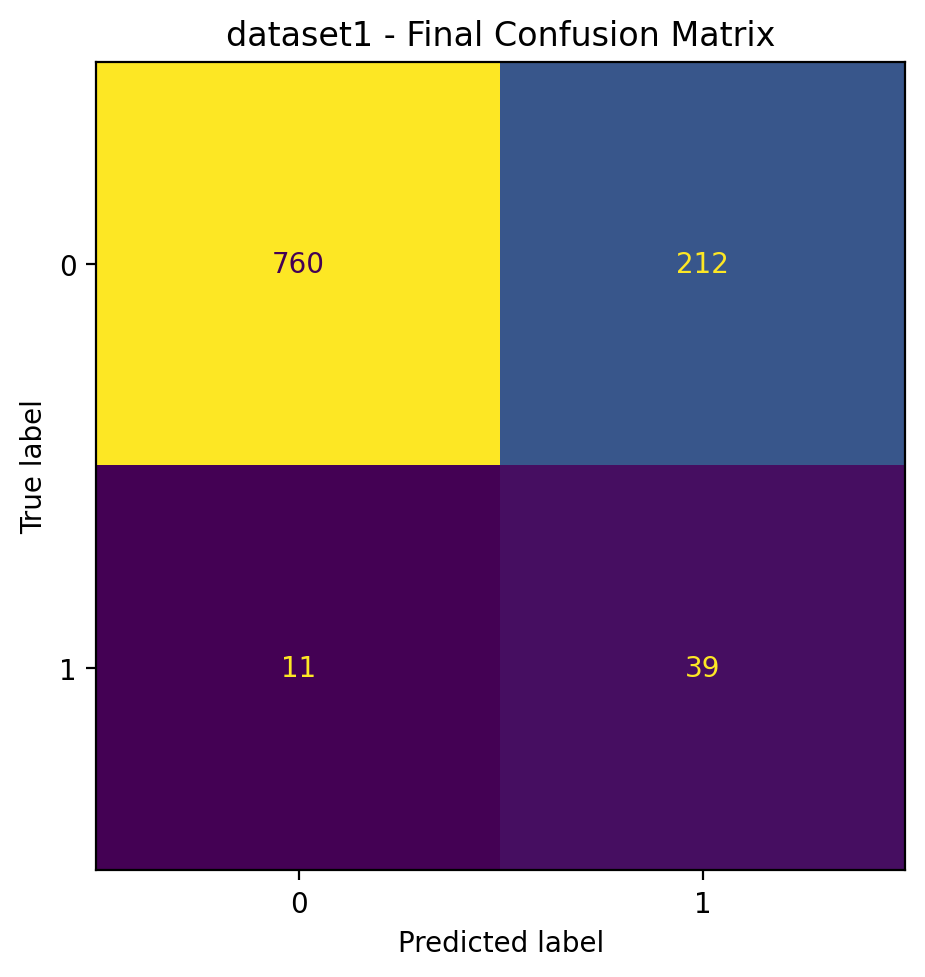
\includegraphics[height=6cm, keepaspectratio]{figures_original/ds1-final_confusion_matrix.png}
	\end{minipage}
	\hfill
	\begin{minipage}[b]{0.48\textwidth}
		\centering
		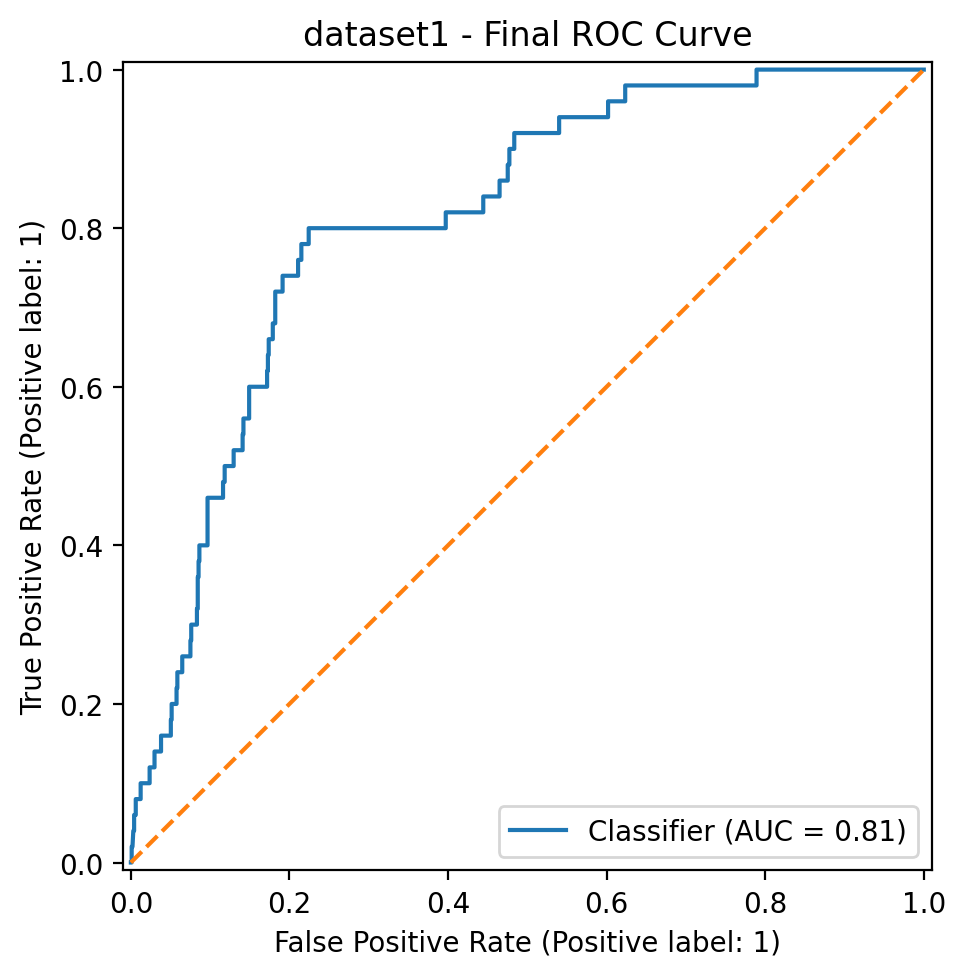
\includegraphics[height=6cm, keepaspectratio]{figures_original/ds1-final_roc_curve.png}
	\end{minipage}
	
	\vspace{0.2cm} % Khoảng cách giữa ảnh và chú thích
	
	% === HÀNG 2: THẲNG HÀNG ĐỈNH CHỮ CHO CAPTION ===
	\begin{minipage}[t]{0.48\textwidth}
		\centering
		\caption{Ma trận nhầm lẫn của mô hình cuối cùng - Dataset 1}
		\label{fig:ds1-final_confusion_matrix}
	\end{minipage}
	\hfill
	\begin{minipage}[t]{0.48\textwidth}
		\centering
		\caption{Đường cong ROC-AUC của mô hình cuối cùng - Dataset 1}
		\label{fig:ds1-final_roc_curve}
	\end{minipage}
\end{figure}
\end{frame}

\begin{frame}{10.2. Kết quả mô hình cuối cùng trên tập kiểm tra - Dataset 2}
	%dataset 1- confusion x roc
	\begin{figure}[H]
		\centering
		% === HÀNG 1: HIỂN THỊ 2 ẢNH CÓ CÙNG CHIỀU CAO (ÉP CÂN BẰNG) ===
		\begin{minipage}[b]{0.48\textwidth}
			\centering
			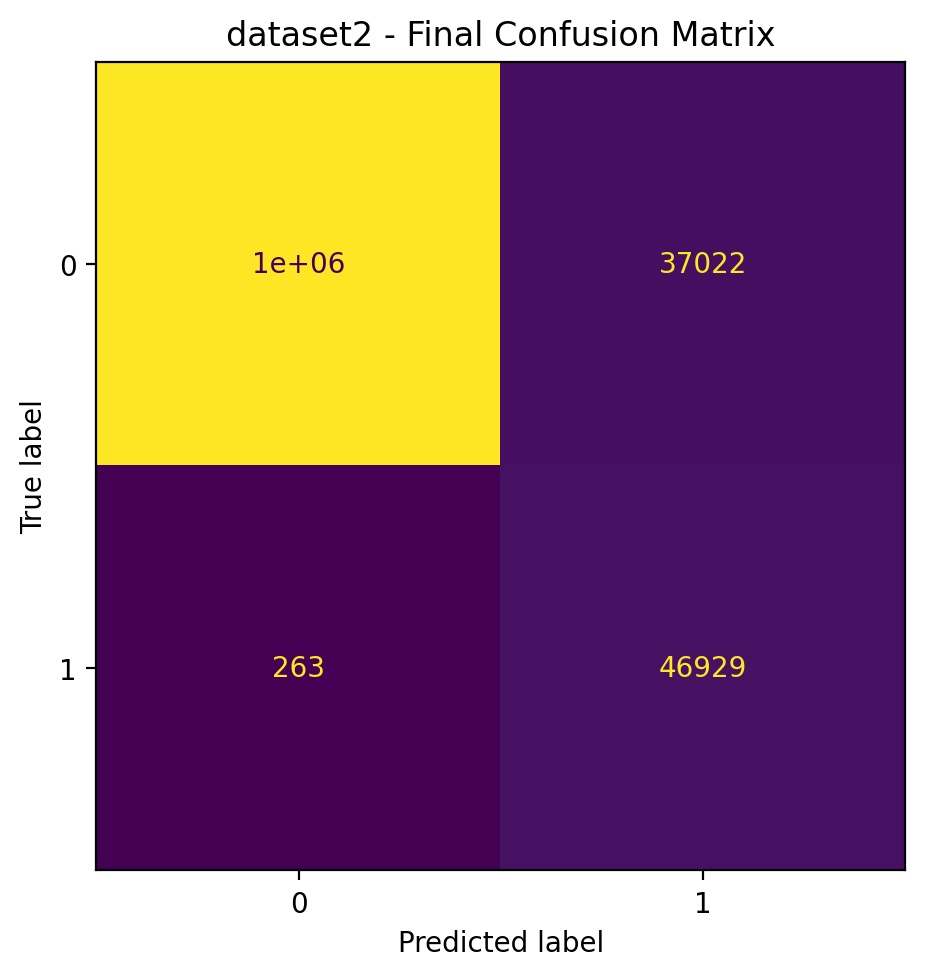
\includegraphics[height=6cm, keepaspectratio]{figures_original/ds2-final_confusion_matrix.png}
		\end{minipage}
		\hfill
		\begin{minipage}[b]{0.48\textwidth}
			\centering
			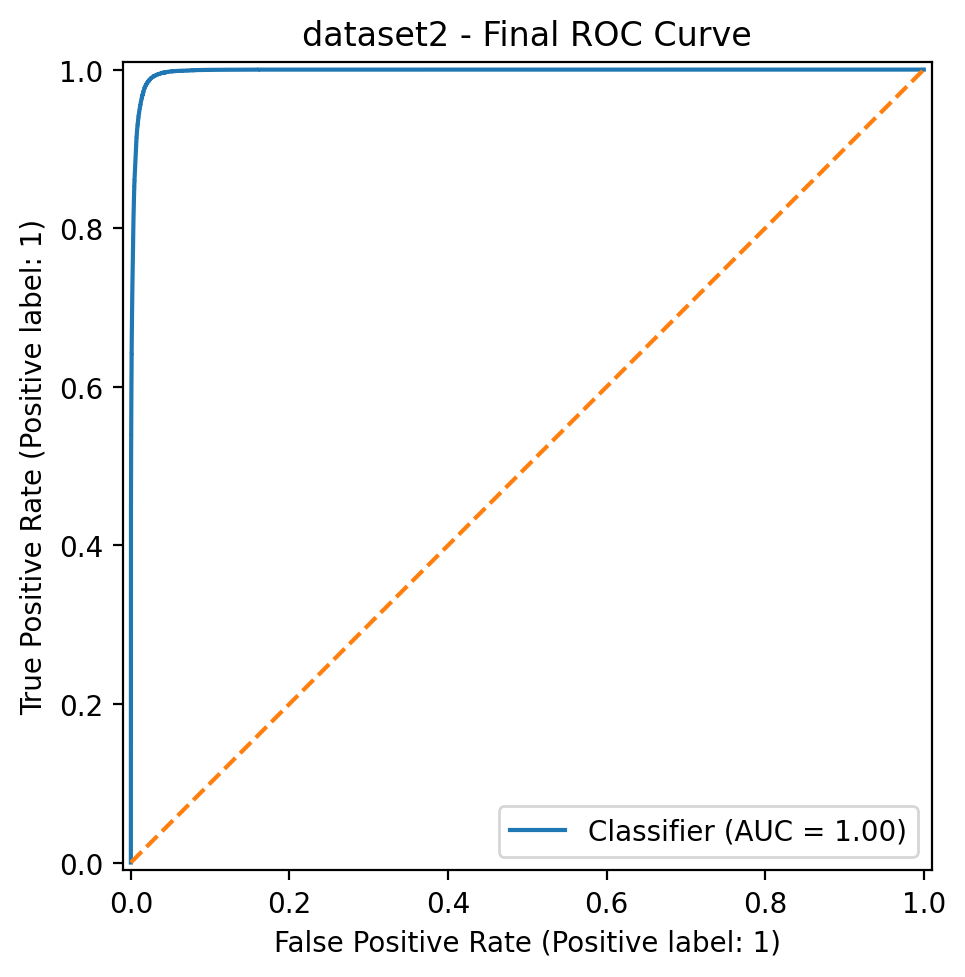
\includegraphics[height=6cm, keepaspectratio]{figures_original/ds2-final_roc_curve.png}
		\end{minipage}
		
		\vspace{0.2cm} % Khoảng cách giữa ảnh và chú thích
		
		% === HÀNG 2: THẲNG HÀNG ĐỈNH CHỮ CHO CAPTION ===
		\begin{minipage}[t]{0.48\textwidth}
			\centering
			\caption{Ma trận nhầm lẫn của mô hình cuối cùng - Dataset 2}
			\label{fig:ds2-final_confusion_matrix}
		\end{minipage}
		\hfill
		\begin{minipage}[t]{0.48\textwidth}
			\centering
			\caption{Đường cong ROC-AUC của mô hình cuối cùng - Dataset 2}
			\label{fig:ds2-final_roc_curve}
		\end{minipage}
	\end{figure}
\end{frame}

\begin{frame}{11. SHAP: mô hình dự đoán dựa vào đâu? - Dataset 1}
	\begin{columns}[T]
		% --- CỘT TRÁI ---
		\begin{column}{0.48\textwidth}
			\centering
			\figmaybe{figures_original/ds1-shap_projected_original_beeswarm.png}{0.95\linewidth}\\
			\vspace{0.1cm}
			\small SHAP Beewarm -- Dataset 1
		\end{column}
		
		% --- CỘT PHẢI ---
		\begin{column}{0.48\textwidth}
			\centering
			\figmaybe{figures_original/ds1-shap_projected_original_bar.png}{0.95\linewidth}\\
			\vspace{0.1cm}
			\small SHAP Bar -- Dataset 1
			
			\vspace{0.1cm} % Khoảng cách vừa phải đẩy khối lưu ý xuống dưới hình
			
			% --- KHỐI LƯU Ý GÓC PHẢI ---
			\begin{flushright}
				\begin{minipage}{0.95\linewidth} % Thu hẹp chiều rộng khối để vừa vặn mép phải
					\begin{block}{Nhận xét}
						\small Mức glucose máu trung bình, tuổi, BMI có ảnh hưởng lớn nhất đến dự báo.
					\end{block}
				\end{minipage}
			\end{flushright}
		\end{column}
	\end{columns}
\end{frame}

\begin{frame}{11. SHAP: mô hình dự đoán dựa vào đâu? - Dataset 2}
	\begin{columns}[T]
		% --- CỘT TRÁI ---
		\begin{column}{0.48\textwidth}
			\centering
			\figmaybe{figures_original/ds2-shap_projected_original_beeswarm.png}{0.95\linewidth}\\
			\vspace{0.1cm}
			\small SHAP Beewarm -- Dataset 2
		\end{column}
		
		% --- CỘT PHẢI ---
		\begin{column}{0.48\textwidth}
			\centering
			\figmaybe{figures_original/ds2-shap_projected_original_bar.png}{0.95\linewidth}\\
			\vspace{0.1cm}
			\small SHAP Bar -- Dataset 2
			
			\vspace{0.1cm} % Khoảng cách vừa phải đẩy khối lưu ý xuống dưới hình
			
			% --- KHỐI LƯU Ý GÓC PHẢI ---
			\begin{flushright}
				\begin{minipage}{0.95\linewidth} % Thu hẹp chiều rộng khối để vừa vặn mép phải
					\begin{block}{Nhận xét}
						\small Mức glucose máu trung bình, tuổi, BMI có ảnh hưởng lớn nhất đến dự báo.
					\end{block}
				\end{minipage}
			\end{flushright}
		\end{column}
	\end{columns}
\end{frame}

\begin{frame}{12. OpenMP và tốc độ (thuật toán Jacobi)}
\small
\begin{tabular}{lrrrrr}\toprule
\textbf{Kích thước ma trận $N$} & 100 & 200 & 300 & 400 & 500\\\midrule
Tuần tự (s) & 0,0441 & 0,2521 & 0,9019 & 2,0456 & 4,0797\\
OpenMP (s) & 0,0731 & 0,2733 & 0,8323 & 1,6355 & 2,6504\\
Speedup & 0,604 & 0,923 & \textbf{1,084} & \textbf{1,251} & \textbf{1,539}\\
\bottomrule\end{tabular}
\vspace{0.7em}
\begin{itemize}
  \item $N=100$ và $N=200$: OpenMP \textbf{chưa} có lợi thế (overhead song song hóa lớn hơn lợi ích).
  \item Từ $N=300$ trở đi: OpenMP bắt đầu nhanh hơn, khoảng cách tăng dần theo kích thước ma trận.
  \item Kết luận: song song hóa chỉ có lợi khi kích thước bài toán đủ lớn, không phải lúc nào cũng nhanh hơn.
\end{itemize}
\end{frame}

\begin{frame}{12. OpenMP và tốc độ (thuật toán Jacobi)}
	\begin{columns}[T]
		% --- CỘT TRÁI ---
		\begin{column}{0.48\textwidth}
			\centering
			\figmaybe{figures_original/execution_time.png}{1\linewidth}\\
			\vspace{0.1cm}
			\small Thời gian thực thi Jacobi theo kích thước ma trận
		\end{column}
		
		% --- CỘT PHẢI ---
		\begin{column}{0.48\textwidth}
			\centering
			\figmaybe{figures_original/openmp_speedup.png}{1\linewidth}\\
			\vspace{0.1cm}
			\small Speedup của OpenMP so với phiên bản tuần tự
		\end{column}
	\end{columns}
\end{frame}


\begin{frame}{13. Thiết kế code tái hiện}
\begin{itemize}
  \item Train/test = 80/20, stratified theo biến mục tiêu.
  \item IQR bounds học từ train rồi áp cho test (tránh rò rỉ dữ liệu).
  \item Sampler (SMOTE/undersampling) và PCA nằm trong \texttt{imblearn.Pipeline}, chỉ fit trên phần train của mỗi fold.
  \item So sánh: baseline (không PCA), sau cân bằng lớp + tinh chỉnh siêu tham số, có/không PCA.
  \item Đánh giá hai bước: kiểm định chéo 10-fold, sau đó một lần hold-out cuối cùng.
  \item Xuất tự động: metrics, confusion matrix, ROC, PCA (cumulative variance, loadings), SHAP.
\end{itemize}
\end{frame}

\begin{frame}{14. Kết luận}
\begin{itemize}
  \item XGBoost + PCA + XAI là pipeline hợp lý cho bài toán dự đoán đột quỵ.
  \item PCA cải thiện có ý nghĩa thống kê trên Dataset 2 (dữ liệu lớn) nhưng lại làm giảm nhẹ accuracy trên Dataset 1 (dữ liệu nhỏ) -- lợi ích phụ thuộc quy mô dữ liệu.
  \item Accuracy cao có thể gây hiểu lầm trên dữ liệu mất cân bằng mạnh; cần xem cùng Precision, Recall, ROC-AUC, MCC.
  \item SHAP giúp diễn giải (glucose, tuổi, BMI là yếu tố nổi bật) nhưng không thay thế kiểm định lâm sàng.
  \item Mục tiêu thực nghiệm: \textbf{tái hiện và đối chiếu}, không giả định sẽ khớp tuyệt đối số liệu bài báo gốc.
\end{itemize}
\end{frame}

\end{document}
